\documentclass[twocolumn]{article}

\usepackage{graphicx}
\usepackage{tikz}
\usepackage{latexsym}

\begin{document}

\title{\textit{In Silico} Separation of Host and Graft Derived Sequence Reads in Xenograft Samples}

\author{
    Thomas Conway\footnote{to whom correspondence should be addressed} \and
    Jeremy Wazny \and
    Andrew Bromage \and
    Bryan Beresford-Smith \and
    Elizabeth Williams}

\date{December 2011}

\maketitle

\begin{abstract}
The interpretation of high throughput, short read sequencing data derived from
xenografts is confounded by the presence of host material in the graft sequence.
We show that a straight-forward analysis using \textit{tophat}
can \textit{in silico} separate sequence
reads in to those most likely derived from the graft, those most likely derived from the host,
those whoes origin is indeterminant, and those that cannot be classified into any of these.
We show that a tool \textit{xenome} we have built can do a more sensitive analysis.
These techniques are demonstrated on sequence data from a human prostate tumor grown in
mice.
The results we present show that the \textit{in silico} analysis is sufficiently
precise and accurate that complicated protocols to perform the separation \textit{in vitro} 
are unnecessary.
\end{abstract}

\section{Introduction}

\section{Methods}

We present two methods for partitioning reads according to whether they
arise from host material or graft material.
The first, uses \texttt{tophat} to analyze the reads with respect to the host reference
and the graft reference, then classifies each read as belonging to host only,
graft only, both, or neither.
The second, \texttt{xenome} using a $k$-mer decomposition of the two reference sequences
is described below.

\subsection{Partitioning with Tophat}
\label{sec:tophat}

\subsection{Xenome}
\label{sec:xenome}

\begin{figure}
\label{fig:venn}
\caption{A Venn diagram showing the different classes that a given $k$-mer may
belong to.
The marginal host and graft partitions are for those host (and graft) $k$-mers
that are Hamming distance 1 from a $k$-mer in the graft (and host) reference.}
\begin{center}
\includegraphics[scale=0.7]{venn.pdf}
\end{center}
\end{figure}

Our method proceeds in two phases: constructing a reference data
structure, then classifying reads with respect to the reference data
structure.  The reference data structure is constructed from a pair of
reference sequences, which we will refer to as the \textit{host} and
the \textit{graft}.

\subsection{Definitions}
\label{sec:xenome:defs}

Consider a $k$-mer $x$. We denote its reverse complement $\bar{x}$.

A canonical $k$-mer $\hat{x}$ is defined given hash function $f$:
$$
\hat{x} =
\left\{
    \begin{array}{ll}
        x       & \mbox{if } \textit{f}(x) < \textit{f}(\bar{x}) \\
        x       & \mbox{if } \textit{f}(x) = \textit{f}(\bar{x}) \mbox{ and } x \le \bar{x} \\
        \bar{x} & \mbox{if } \textit{f}(x) = \textit{f}(\bar{x}) \mbox{ and } x > \bar{x} \\
        \bar{x} & \mbox{if } \textit{f}(x) > \textit{f}(\bar{x})
    \end{array}
\right.
$$

We say that a $k$-mer is \textit{marginally} distinctive if it exists in just one of the two genomes
but has a Hamming distance 1 neighbour in the other genome. We therefore define
the following Boolean function:
$$
\mathcal{M}(x, S) =
\left\{
    \begin{array}{ll}
        \mathit{true} & \mbox{if } \exists y : y \in \textit{Ham}_1(x)
                      \wedge y \in S    \\
        \mathit{false} & \mbox{if } \forall y : y \in \textit{Ham}_1(x)
                      \wedge y \notin S  \\
    \end{array}
\right.
$$
where $\textit{Ham}_1(x)$ is the set of Hamming distance one neighbours
of $x$.

\subsection{Reference Construction}

For each reference sequence we construct the set of
canonical $k$-mers ($\hat{H}$ and $\hat{G}$ respectively).  From these
we compute a complete set of canonical reference $k$-mers
$\hat{S} = \hat{H} \cup \hat{G}$
(Note that $\forall x \in \hat{S}, x = \hat{x}$).

\begin{table}
\label{tbl:class}
\begin{center}
\begin{tabular}{l|c|c}
                & $x \in \hat{H}$ & $x \notin \hat{H}$  \\
\hline
$x \in \hat{G}$   & $11$      & $\begin{array}{l} 00 \mbox{ if } \mathcal{M}(x, \hat{H}) \\
                                                                  01 \mbox{ otherwise} \end{array}$              \\
\hline
$x \notin \hat{G}$& $\begin{array}{l} 00 \mbox{ if } \mathcal{M}(x, \hat{G}) \\
                                                  10 \mbox{ otherwise} \end{array}$ & $\bot$       \\
\end{tabular}
\end{center}
\caption{A table showing how the 2-bit class number of each $k$-mer is computed where $\hat{G}$ is the set of canonical
$k$-mers from the graft reference, $\hat{H}$ is the set of canonical $k$-mers from the host reference and $\mathcal{M}$
is the boolean function defined in \ref{sec:xenome:defs} that defines \textit{marginal} inclusion.}
\end{table}

For each $x \in \hat{S}$, we compute a 2-bit class $c_x$ as shown
in Table~\ref{tbl:class}.  The bit pair $00$ denotes $k$-mers either
from the host or graft genome that have a near (Hamming distance one)
neighbour in the other genome: they are \textit{marginally} distinctive,
in the sense that a single polymorphism or sequencing error may cause
a $k$-mer in that class to change from being marginally host to begin
marginally graft.  Since the marginal set is symmetric (every marginal
host $k$-mer has a corresponding marginal graft $k$-mer, and vice versa),
and represents $k$-mers that are not very discriminating, we combine
both marginal sets into a single marginal set with the class $00$.

\begin{table}
\label{tbl:classes}
\begin{center}
\begin{tabular}{|cccc|l|}
\hline
\multicolumn{4}{|c|}{$k$-mer class} & read class \\
$01$        & $10$      & $11$  & $00$ & \\
\hline
$\bullet$   & $\circ$   &    $\ast$ &    $\ast$ & \textit{graft}          \\
$\circ$     & $\bullet$ &    $\ast$ &    $\ast$ & \textit{host}           \\
$\circ$     & $\circ$   & $\bullet$ &    $\ast$ & \textit{both}           \\
$\circ$     & $\circ$   & $\circ$   & $\bullet$ & \textit{both}           \\
$\bullet$   & $\bullet$ &    $\ast$ &    $\ast$ & \textit{ambiguous}      \\
$\circ$     & $\circ$   & $\circ$   &   $\circ$ & \textit{neither}        \\
\hline
\end{tabular}
\caption{The mapping of $k$-mer classes to read classifications.
$\bullet$ denotes cases where the $k$-mer class is present, $\circ$ where the $k$-mer class is absent,
and $\ast$ where the $k$-mer class may be either present or absent.}
\end{center}
\end{table}

\subsection{Classification}

Classification proceeds by taking each read $r$ and constructing the set
of canonical $k$-mers that may be derived from the read $\hat{Q}_r$. We
then map the $k$-mers to classes using the mapping described above,
and classify the read based on the set of $k$-mer classes as described
in table~\ref{tbl:classes}.  The read classes \textit{graft} and
\textit{host} denote cases where there is at least one $k$-mer which
unambiguously comes from that $k$-mer class, and there are no contradictory
$k$-mers (i.e. unambiguously from the opposing reference).
The \textit{ambiguous} class corresponds to the case where there
are $k$-mers which appear to be contradictory --- unambiguously host,
and unambiguously graft. The \textit{both} class represents cases where
there are only $k$-mers which are either unambiguously common to both the
host and graft, or $k$-mers which may belong to either if they contain a
single polymorphism or sequencing error. The last class, \textit{neither}
represents those cases where there were no matching $k$-mers.


\section{Results}

We wish to perform analysis to establish two things: that it is technically
feasible to separate host and graft reads \textit{in silico}; and that the
fast technique we have proposed does so with at least comparable accuracy
to other methods.

\begin{figure}
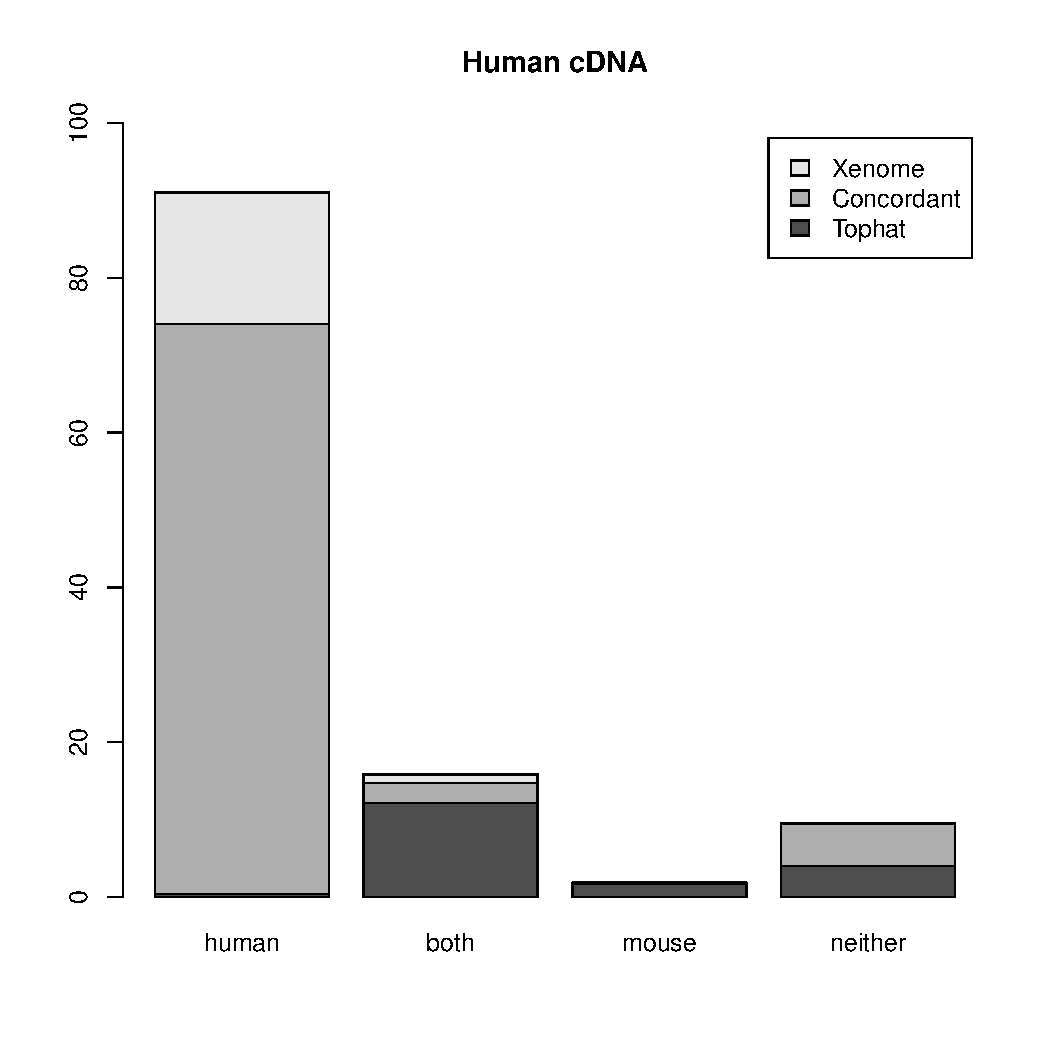
\includegraphics[scale=0.4]{human.pdf}
\caption{Summary of the results with Human cDNA.}
\label{fig:human}
\end{figure}

\begin{figure}
\includegraphics[scale=0.4]{mouse.pdf}
\caption{Summary of the results with Mouse cDNA.}
\label{fig:mouse}
\end{figure}

\begin{figure}
\includegraphics[scale=0.4]{bm18-26.pdf}
\caption{Summary of the results with BM18 xenograft cDNA.}
\label{fig:bm18}
\end{figure}

To this end, we present the results of two experiments. In the first, we take a sample of
human cDNA sequence data (SRR342886), and a sample of mouse cDNA sequence data (SRR037689)
and analyse them both with Tophat\cite{tophat} and Xenome, and compare the results.
The second experiment takes sequence data from a human prostate cancer/mouse xenograft,
runs the same comparitive analysis, and uses QPCR on selected genes to validate the results.

Tophat is a global analysis, using the results of all the read mappings to
locate splice sites, fusions, and so on. By contrast, Xenome, performs
pre-computation on the two reference genomes, then classifies each
read independently. Therefore the comparative analysis is conducted
by running the sample reads with Tophat against the human genome and
against the mouse genome. Reads are then classified as \textit{human},
\textit{both}, \textit{mouse} or \textit{neither} according to the results of Tophat.
Then, each group of reads is run through Xenome, which classifies reads into
the five groups described in section \ref{sec:xenome}.
For the purposes of comparison, we tread reads classed by Xenome as \textit{ambiguous}
the same as reads classed by the Tophat analysis as \textit{both}.
Figures \ref{fig:human} and \ref{fig:mouse} summarise the results. In both figures,
there is a bar for each of the classes with three parts. The middle part represents
the number of reads for which the Tophat analysis and Xenome analysis produced the same
assignment. Below it is a part depicting the number of reads assigned to that class
by the Tophat analysis, but not the Xenome analysis; and above the middle bar is a part
depicting the number of reads assigned to that class by Xenome but not the Tophat analysis.

In this experiment, there is very little cross-talk --- reads of human origin showing up as
mouse but not human, and reads of mouse origin showing up as human but not mouse
(on the mouse data, both tools show about 0.2\% classed as human, a similar number for
Xenome on the human data, with Tophat assigning about 1.7\% of the human data to mouse).
On both data sets, both tools correctly classified most reads, but in both cases, Xenome
correctly classified about 10\% more reads unambiguously.
In both samples, the Tophat analysis was more likely to class a read as being possibly
either human or mouse in origin: 14.7\% and 7.8\% for human and mouse respectively,
versus 3.1\% and 0.6\% for Xenome.
Both tools largely agreed on which reads were unclassifiable (neither).

These results strongly suggest that separation of reads is feasible, and that Xenome
is more sensitive than the Tophat based approach.

In the second experiment, we have taken experimental data from a prostate cancer
xenograft into a mouse and performed the same procedure. In addition, we have computed
relative expression levels for selected genes by counting numbers of reads and
normalizing for the span covered by the reads.
We have then validated these expression levels with QRT-PCR with human specific primers.

%Mouse RNA
%
%\begin{tabular}{|r|rrrrr|rr|}
%\hline
%        & Xenome    &           &           &           &           & Total     & \\
%Tophat  & Human     & Both      & Mouse     & Neither   & Ambiguous &           & \\
%\hline
%Human   &     5,028 &     2,115 &    27,188 &     1,143 &     1,709 &    37,183 &  0.2\%   \\
%Both    &    14,103 &    38,672 & 1,145,894 &     6,034 &    21,680 & 1,226,383 &  7.8\%   \\
%Mouse   &     6,933 &    25,147 &11,920,029 &   288,523 &    37,225 &12,277,857 & 77.9\%   \\
%Neither &    10,324 &    28,404 &   526,413 & 1,649,259 &     4,204 & 2,218,604 & 14.1\%   \\
%\hline
%Total   &    36,388 &    94,338 &13,619,524 & 1,944,959 &    64,818 &15,760,027 &          \\
%Total   &    0.2\%  &    0.6\%  & 86.4\%    & 12.3\%    &    0.4\% &            &          \\
%\hline
%\end{tabular}

%\begin{tikzpicture}[xscale=0.075, yscale=0.5]
%    % Human
%    \fill[blue] (-0.347,0) rectangle (-0.025,1) ;
%    \fill[gray] (-0.025,0) rectangle (0.025,1) ;
%    \fill[red]  (0.025,0) rectangle (0.339,1) ;
%
%    % Both
%    \fill[blue] (-11.962,2) rectangle (-0.302,3) ;
%    \fill[gray] (-0.302,2) rectangle (0.302,3) ;
%    \fill[red]  (0.302,2) rectangle (1.290,3) ;
%
%    % Mouse
%    \fill[blue] (-63.178,4) rectangle (-59.600,5) ;
%    \fill[gray] (-59.600,4) rectangle (59.600,5) ;
%    \fill[red] (59.600,4) rectangle (76.595,5) ;
%
%    % Neither
%    \fill[blue] (-13.940,6) rectangle (-8.246,7) ;
%    \fill[gray] (-8.246,6) rectangle (8.246,7) ;
%    \fill[red] (8.246,6) rectangle (11.203,7) ;
%\end{tikzpicture}

%Human RNA
%
%\begin{tabular}{|r|rrrrr|rr|}
%\hline
%        & Xenome    &           &           &           &           & Total     &           \\
%Tophat  & Human     & Both      & Mouse     & Neither   & Ambiguous &           &           \\
%\hline
%Human	&21,709,447 &    22,732 &     2,263 &    14,407 &    71,580	&21,820,429	& 74.03\%   \\
%Both	& 3,558,106	&   685,377 &    21,325 &     1,028	&    78,277	& 4,344,113	& 14.74\%   \\
%Mouse	&   314,353	&   188,712 &     8,620	&       308	&     7,092	&   519,085	& 1.76\%	\\
%Neither	& 1,128,193	&    22,192	&     3,772	& 1,620,702	&    18,456	& 2,793,315	& 9.48\%	\\
%\hline
%Total   &26,710,099	&   919,013	&    35,980 & 1,636,445	&   175,405	&29,476,942	&           \\
%	    & 90.61\%	& 3.12\%	& 0.12\%    & 5.55\%	& 0.60\%	&           &           \\
%\hline
%\end{tabular}


%Since we are particularly interested in applying our technique to cancer
%research where human cancer cells are grafted into mice, we have tested
%our technique using the human genome as the graft reference, and
%the mouse genome as the host reference.
%For classification,
%we have used a set of experimental reads derived from a human cDNA sample,
%and a set of experimental reads derived from a mouse cDNA sample.
%In each case, an ideal analysis should class every read as \textit{both}
%or one of human or mouse respectively.
%Of course, we expect some level of cross-talk due to genetic variation
%(polymorphism) and sequencing errors, and that is precisely what we want
%to evaluate.
%
%To evaluate the relative sensitivity and accuracy of our method we have compared
%our technique with the straight-forward classifications that result from
%the alignments against the human and mouse genomes
%using \texttt{stampy} (which uses \texttt{bwa} internally
%to improve performance).
%We believe it is better to align to the reference genome, rather than a
%reference transcriptome, because, although splicing may lead to problems,
%so do events such as read-throughs, in which a transcript contains intronic
%sequence. The reference genome is also more likely to capture novel transcripts
%that are not among the established reference set.
%
%The alignment based classification proceeds by aligning the set of reads
%against the two reference genomes and  comparing the results to classify
%reads as belonging to one or the other genome, both or neither. This
%method conflates the \textit{ambiguous} and \textit{both} classes of
%our technique.
%In many cases, the alignment programs are able to generate an alignment,
%even though the likelihood of the alignment being true is low.
%Thus in comparing the alignments against the human and mouse genomes,
%we have used the mapping quality to filter alignments to eliminate
%ones of low quality (PHRED score less than 30).
%
%Our evaluation is performed using the human (hg19) and mouse (NCBIM37)
%genomes.  We have taken to publicly available data sets of human and
%mouse transcriptome data (ERX011226 and SRX017602 respectively) to allow
%us to evaluate the accuracy of our method.
%
%For each of the data sets we have performed a classification by our method
%and using mappings created by each of \texttt{bwa} and \texttt{stampy}.
%
%Table \ref{tbl:main} presents these results.
%
%\begin{table}
%\caption{Results of comparing xenome with mapping.}
%\begin{tabular}{|rr|rrrr|rrrr|}
%\multicolumn{2}{c}{xenome} & \multicolumn{4}{c}{\texttt{bwa}} & \multicolumn{4}{c}{\texttt{stampy}} \\ \hline
%\multicolumn{10}{c}{human transcriptome} \\ \hline
%          & total & mouse & both & human & neither & mouse & both & human & neither \\
%mouse     &       &   0 &     0 &     0 &     0 &     0 &     0 &     0 &     0 \\
%both      &       &   0 &     0 &     0 &     0 &     0 &     0 &     0 &     0 \\
%human     &       &   0 &     0 &     0 &     0 &     0 &     0 &     0 &     0 \\
%neither   &       &   0 &     0 &     0 &     0 &     0 &     0 &     0 &     0 \\
%ambiguous &       &   0 &     0 &     0 &     0 &     0 &     0 &     0 &     0 \\ \hline
%(total)   &           &   0 &     0 &     0 &     0 &       0 &       0 &      0 &         0 \\ \hline
%\multicolumn{10}{c}{mouse transcriptome} \\ \hline
%          & total & mouse & both & human & neither & mouse & both & human & neither \\
%mouse     &       &   0 &     0 &     0 &     0 &   0     &     0   &     0  &     0 \\
%both      &       &   0 &     0 &     0 &     0 &   0     &     0   &     0  &     0 \\
%human     &    36,388 &   0 &     0 &     0 &     0 &   1,273 &  30,865 &  2,446 &     1,804 \\
%neither   & 1,768,829 &   0 &     0 &     0 &     0 & 590,092 & 159,203 & 18,534 & 1,001,000 \\
%ambiguous &    64,818 &   0 &     0 &     0 &     0 &   5,984 &  58,431 &     95 &       308 \\ \hline
%(total)   &           &   0 &     0 &     0 &     0 &       0 &       0 &      0 &         0 \\ \hline
%\end{tabular}
%\end{table}
%
%\section{Discussion}
%
%Our method relies on the fact that as $k$ increases,
%$k$-mers become increasingly likely to be specific to a single species.
%On the other hand, as $k$ increases, a given $k$-mer in a read is increasingly
%likely to contain a polymorphism or a sequencing error. The sparseness of
%the $k$-mer space means that divergent $k$-mers are overwhelmingly likely
%to be novel (not occurring in either reference).
%
%\begin{figure}
%\label{fig:mapq}
%\caption{A histogram showing the distribution of differences in \texttt{stampy}
%mapping quality for reads from the mouse transcriptome judged by \texttt{xenome} to 
%be of mouse origin.}
%\begin{center}
%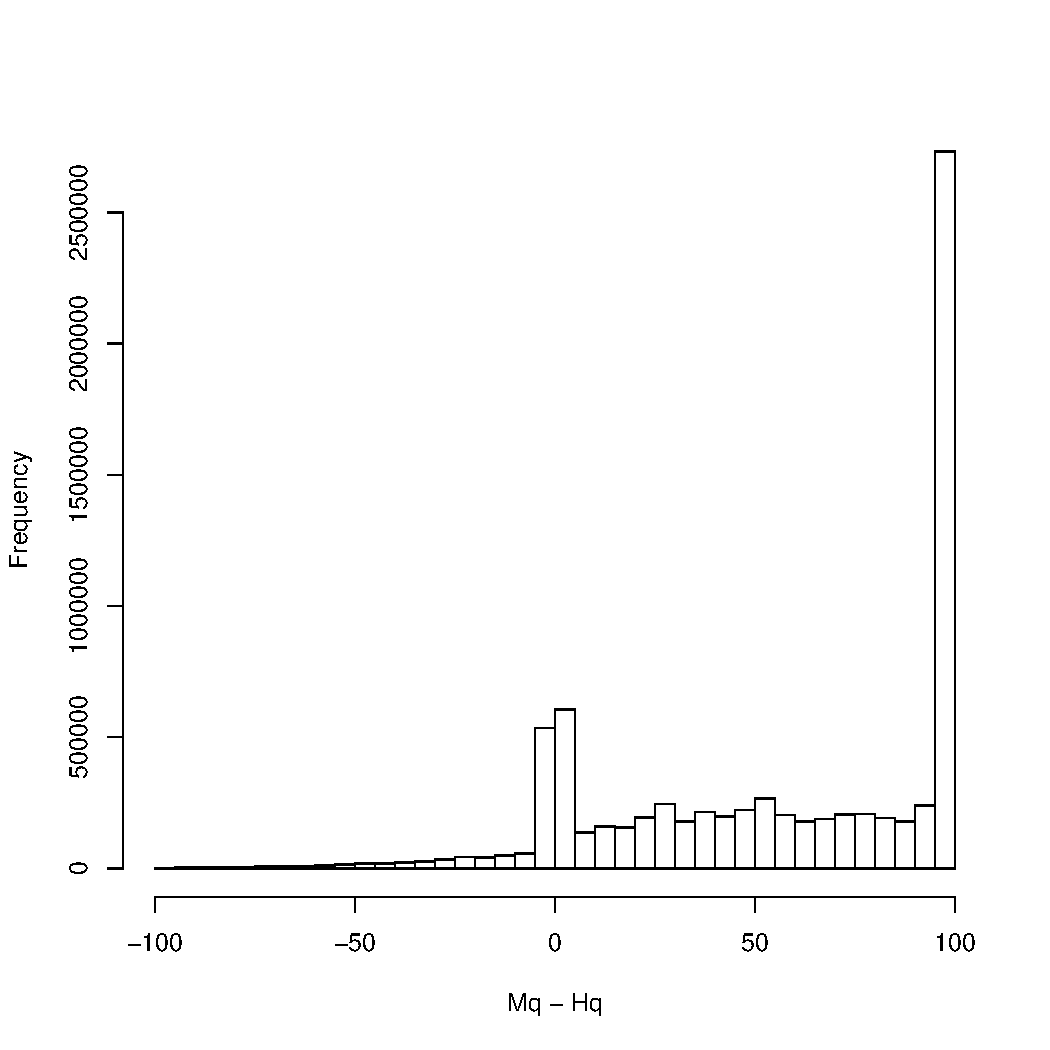
\includegraphics[scale=0.4]{mapqual-hist.pdf}
%\end{center}
%\end{figure}
%
%If we consider the fraction of the mouse transcriptome reads that \texttt{xenome}
%assigns to being mouse specific,
%there is an important detail to consider with respect to the analysis of
%the results of mapping with \texttt{stampy}.
%It assigns a mapping quality score in the range $[0, 100]$,
%in the manner of a PHRED score.
%
%Figure~\ref{fig:mapq} shows, this data, a histogram of the difference in mapping
%quality score for reads that successfully mapped to both the human and mouse genomes
%(and would naively fall in the \textit{both} class of read assignments).
%It is clear that most of the time, the mouse mapping quality is high and the human
%mapping quality is low --- in such a case we should really assign such reads to the
%\textit{mouse-only} class.
%Of the rest, the most frequent case is that both mappings have low
%quality, and therefore the corresponding reads should be assigned to the
%\textit{neither} class, or that both mappings have high quality and the
%corresponding reads should be assigned to the \textit{both} class.
%These two cases are not obviously distinguished in the histogram, but are readily
%apparent when looking at the quality scores themselves.
%
%There is a significant minority where there is an intermediate score for both mappings,
%though almost always the mouse mapping has a higher quality score than the human one.


\end{document}
